\chapter{Сначала успокоение, потом реформы}


Нельзя навеки застыть в одном положении. Время всегда будет идти вперед, изменяя мир и принося за собой новые проблемы, которые всё больше будут накапливаться и всё сильнее толкать людей к переменам, как бы они не цеплялись за старый мир.

Зима 1905 года показала то, что Россию постиг кризис. Кризис этот сформировался вокруг двух вещей: «земля и воля». У множества людей были свои варианты разрешения кризиса и многие из предлагаемых решений были связаны с пролитием крови. Одной из попыток уйти от баррикад и кровопролития стало создание Государственной Думы Российской империи 1 созыва. Однако, Дума, вобрав в себя людей с самыми разными взглядами, не стала кузницей благоприятных для вышестоящего правительства решений. Наоборот, она стала максимально противоположной действующей власти. В начале июля 1906 года Николай II готовится к роспуску этого госоргана и назначает Петра Столыпина председателем Совета министров («премьер» если по-простому). Столыпин начинает готовиться к ухудшению ситуации и рассылает телеграммы по губерниям с требованием пресекать любую антиправительственную пропаганду. Думу распускают на семь месяцев, в течение которых должны пройти новые выборы.

Депутаты, в ответ на роспуск, покидают Санкт-Петербург и выпускают «Выборгское воззвание»: по сути, призывая к массовым беспорядкам. Это лишь только первое воззвание из многих, которые бывшие народные избранники собираются выпустить и распространить по империи. Конечно, депутатов арестовывают, но новости об арестах только сильнее разогревают ненависть к власти. По итогу, большинство подписавших воззвание депутатов осудят только на три месяца заключения в «Крестах» лишь ради того, чтобы они не смогли участвовать в выборах второго созыва.
Всё это лишь политические стороны проблемы. А по стране в это же время пошла волна недовольства, перетекающая в схватки с полицией и военными. Как пример здесь можно привести Свеаборгское восстание, разгорающееся еще до роспуска Думы.

Также здесь возникают проблемы со статистикой. В своем большинстве все последующие действия выливались не в массовые стычки, восстания и баррикады на улицах, а в одиночные операции. Деяния революционеров были направлены как на убийства конкретных представителей власти (заочно приговорённых к смерти за преступления против народа), так и к грабежам («экспроприации»), задача которых была в пополнении революционной кассы. Многие из этих событий относили к бандитизму и никак не связывали с революционным терроризмом, и сведения о таком публиковались в газетах в обычной криминальной статистике. Аналогичная ситуация и с учетом пострадавших от действий жандармов и казаков – многие данные о погибших имеют под собой источник в виде подпольных газет, но не имеют официального учета. Газета «Биржевые ведомости»,  имеющая тогда нейтральные позиции, указывала на 1100 погибших из-за революционных действий за 1906 год, из которых 410 – это полицейские и военные чины.

Точно можно сказать, что волнения только усиливались и уже зацепили Столыпина. В августе при помощи бомб в портфелях совершается атака на приемную премьера, расположенная на государственной даче. Погибло 27 человек, пострадали дети Столыпина. Ответ террористам был жестким: в России ввели военно-полевые суды.

Важно отметить, что такой суд распространялся только на губернии, находящиеся «в исключительном положении», практически, на военном положении. Из 87 губерний и областей империи в сентябре 1906 такими стали 82. Военно-полевой суд собирался разово по решению генерал-губернатора или командующего войсками. Суд состоял из пяти строевых офицеров армии или флота с выслугой больше четырех лет, чьи данные не будут раскрываться и учитываться после суда – не велся даже протокол заседания. На военно-полевом суде не присутствовали адвокаты или обвинители. При этом при наборе судей намеренно исключались офицеры военно-судебного ведомства. Задача перед таким судом стояла простая – вынести вердикт и меру наказания, если «учиненное деяние является настолько очевидным, что нет надобности в его расследовании».
\begin{figure}[h!tb] 
	\centering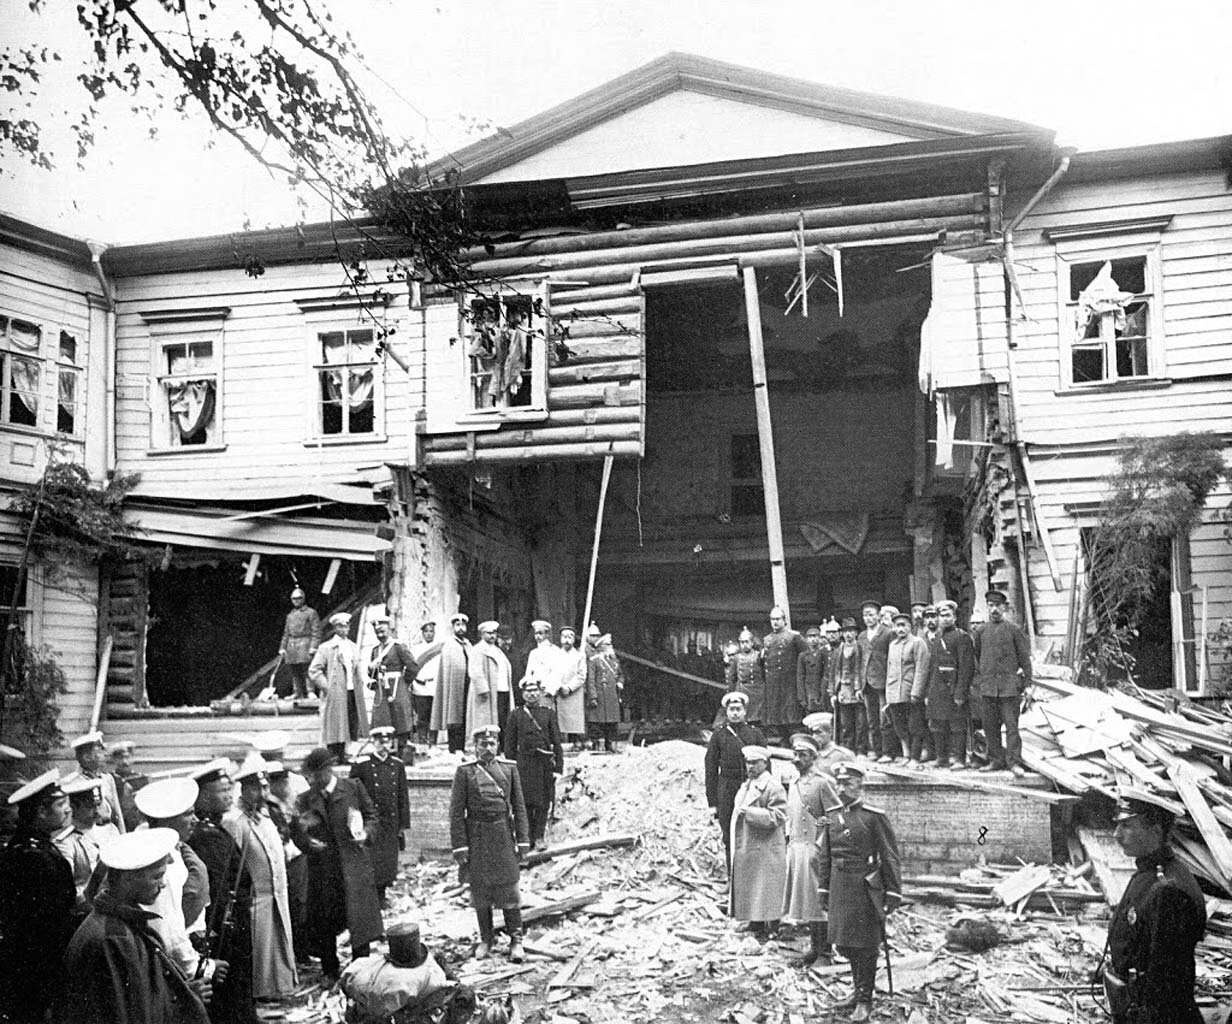
\includegraphics[scale=0.4]{Stolypin2/zU206u1v7wY.jpg}
	%	\label{fig:scipion} % Unique label used for referencing the figure in-text\end{document}
	%	%\addcontentsline{toc}{figure}{Figure \ref{fig:placeholder}} % Uncomment to add the figure to the table of contents%----------------------------------------------------------------------------------------
	%\caption{Если искать в интернете инфу про отца Морлиона, то найдется очень много различной литературы про знаменитых шпионов. Так или иначе, за Морлионом закрепилось звание агента ЦРУ — что, судя по найденной мною инфе, неудивительно. Я не очень в шпионских делах - может, когда-нибудь... }%	CHAPTER 2
\end{figure}
Такой способ создания суда предполагал быстродействие, за счет отсутствия скованности процессуальными действиями, но в итоге привел и к жестокости – за первые два месяца большую часть вердиктов были положительными и выбирали меру наказания в виде смертной казни (меры наказания не были никак прописаны и устанавливались по желанию судьей). Был издан императорский циркуляр, что военно-полевой суд должен рассматривать только дела за последние 48 часов с созыва суда и только тяжёлые дела по отношению к государственным чинам, а также все случаи подготовки терактов.

Несмотря на все политические усилия Столыпина, Дума второго созыва тоже оказалась не так лояльна действующей власти, как хотелось. Депутаты резко осудили практику полевых судов, называя ее нарушением самих идей Империи. И в апреле 1907 года такие суды прекратили свое существование. Опять же, статистика терактов пошла на спад – они всё еще присутствовали, но уже не выбивали то желание решительных мер. А Столыпин снова ушел полностью в политику, решая вопрос лояльности Думы правительству, что должно было позволить совершить реформы.

В итоге летом 1907 будет роспуск и второго созыва Думы. Третий станет гораздо лояльней, но всё еще будет помнить Столыпину его жесткость в подавление революции. Так, адвокат и депутат всех созывов, Федор Родичев в ноябре на заседании сделал следующее заявление: «…в то время, когда русская власть находилась в борьбе с эксцессами революции, только одно средство видели, один палладиум в том, что господин Пуришкевич называет муравьёвским воротником и что его потомки назовут, быть может, столыпинским галстуком».

Муравьёвский воротник – такое название дали веревке виселицы, которой граф Муравьёв-Виленский в своё время подавлял польское восстание 1863 года. Сам Столыпин после такого заявления вызвал Родичева на дуэль, но депутат лично принес извинения и был просто исключен на 15 заседаний из думы.
В журнале «Право» от 1908 года была опубликована статистика итогов действий военно-полевых судов: 1144 смертных приговоров. Это еще к десяткам тысячам каторжников по итогу неудавшейся революции. При этом и обычные суды продолжали выносить смертные приговоры уже новым участникам подпольных ячеек. Публикация вызвала шквал критики со стороны интеллигенции. Да, той самой, которая «*овно» (потому что так Ленин сказал) и которая «вечно обижает русских людей» (да кто так только не говорил). Именно она и заступилась за крестьян, с которыми никто не церемонился и которым никогда не заменяли смертный приговор - ссылкой.
Лучше всего это олицетворяет манифест Льва Николаевича Толстого «Не могу молчать». Вот цитаты оттуда (но рекомендую прочитать манифест целиком):

«Ужаснее же всего в этом то, что все эти бесчеловечные насилия и убийства, кроме того прямого зла, которое они причиняют жертвам насилий и их семьям, причиняют еще большее, величайшее зло всему народу, разнося быстро распространяющееся, как пожар по сухой соломе, развращение всех сословий русского народа. Распространяется же это развращение особенно быстро среди простого, рабочего народа потому, что все эти преступления, превышающие в сотни раз всё то, что делалось и делается простыми ворами и разбойниками и всеми революционерами вместе, совершаются под видом чего-то нужного, хорошего, необходимого, не только оправдываемого, но поддерживаемого разными, нераздельными в понятиях народа с справедливостью и даже святостью учреждениями: Сенат, Синод, Дума, церковь, царь.»
«Недавно еще не могли найти во всем русском народе двух палачей. Еще недавно, в 80-х годах, был только один палач во всей России. Помню, как тогда Соловьев Владимир с радостью рассказывал мне, как не могли по всей России найти другого палача, и одного возили с места на место. Теперь не то». Владимир Сергеевич Соловьёв – поэт и публицист конца 19-го века.
«Сила событий никак не в материальных условиях жизни, а в духовном настроении народа. Если бы вы убили и замучили хотя бы и десятую часть всего русского народа, духовное состояние остальных не станет таким, какого вы желаете.»

Причина такой реакции проста: за один год «политических» смертных приговоров было больше, чем за весь 19-й век. Это шокировало людей. Людей, которые еще не знали сколько крови прольется в стране в будущем.
И Столыпину этого не простили революционеры, убив «обер-вешателя» (так премьера назвал Ленин) в сентябре 1911 года.

История России начала двадцатого века – это не история про рыцарей или еще каких-то символических представителей "всего самого доброго". Это история времени, которое требовало перемен и людей, которым бы пришлось совершить эти перемены, заплатив за них значимую цену. Сейчас можно долго обсуждать «оправдывает ли цель средства», подключая к обсуждению исторических событий обязательно современную политическую повестку, с указанием кто на повестке теперь хороший, а кто плохой. Важно понимание того, что бездействие и мечтание о «авось» и привело страну к той самой точке невозврата, когда проблему уже нельзя решить, не повязав галстуков.

Автор Александр Прохоров. Ссылка \url{https://vk.com/wall-162479647_176990}
\#Прохоров@catx2
\#Заметка@catx2
